\documentclass[11pt]{article}

% --- Packages (The "plugins" of LaTeX) ---
\usepackage[utf8]{inputenc} % Character encoding
\usepackage{geometry}       % Page margins
 \geometry{margin=1in}
\usepackage{graphicx}       % For inserting images
\usepackage{amsmath}        % For math equations
\usepackage{listings}
\usepackage{xcolor} % Required for syntax highlighting colors
\usepackage{booktabs} % For professional lines
\usepackage{siunitx}  % For decimal alignment

% Define colors for Python syntax
\definecolor{codegreen}{rgb}{0,0.6,0}
\definecolor{codegray}{rgb}{0.5,0.5,0.5}
\definecolor{codepurple}{rgb}{0.58,0,0.82}
\definecolor{backcolour}{rgb}{0.95,0.95,0.92}
\definecolor{termback}{rgb}{0.1,0.1,0.1}
\definecolor{termtext}{rgb}{0.9,0.9,0.9}
\definecolor{lightgray}{rgb}{0.9,0.9,0.9}

\lstdefinestyle{mystyle}{
    backgroundcolor=\color{backcolour},   
    commentstyle=\color{codegreen},
    keywordstyle=\color{magenta},
    numberstyle=\tiny\color{codegray},
    stringstyle=\color{codepurple},
    basicstyle=\ttfamily\footnotesize,
    breakatwhitespace=false,         
    breaklines=true,                 
    captionpos=b,                    
    keepspaces=true,                 
    numbers=left,                    
    numbersep=5pt,                  
    showspaces=false,                
    showstringspaces=false,
    showtabs=false,                  
    tabsize=2
}

\lstdefinestyle{terminal}{
    backgroundcolor=\color{white},   % White background
    basicstyle=\ttfamily\small\color{black}, % Black text
    frame=single,                    % Simple border
    rulecolor=\color{lightgray},     % Light gray border color
    breaklines=true,                 % Wrap long lines
    numbers=none,                    % No line numbers for output
    captionpos=b,                    % Caption at the bottom
    xleftmargin=10pt,                
    xrightmargin=10pt,
    framesep=5pt
}

\lstset{style=mystyle}

% --- Document Information ---
\title{DE 414: Practical 4 Report}
\author{Amy McDermott (26911264)}
\date{\today}

\begin{document}

\maketitle

\section*{Introduction}
This report documents the implementation of a Multi-layer Perceptron using Python. It explores the manual application of the forward pass, 
backpropagation, and loss calculation. The model's performance and ability to generalise are tested against the datasets \texttt{simple} and \texttt{two\_blob}. 
By visualising the decision surfaces generated by the model, we can observe how the neural network's architectural choices - such as the number 
of hidden layers and neurons - impacts the network's capacity to handle various levels of data complexity.

\section*{Question 1: Single layer perceptron}
In this section, a single-layer perceptron was implemented and trained on the \texttt{simple} dataset. This architecture consists of 2 input units, $P1 = 3$, and 1 output unit, $Q1 = 1$.
\subsection*{Loading of data}
The first step of the practical involved loading the \texttt{simple} dataset and visualising its distribution. Using the \texttt{matplotlib} library, a scatter plot 
was generated with points colour-coded by their respective labels (red for class 0 and green for class 1).

\begin{figure}[htbp]
    \centering
    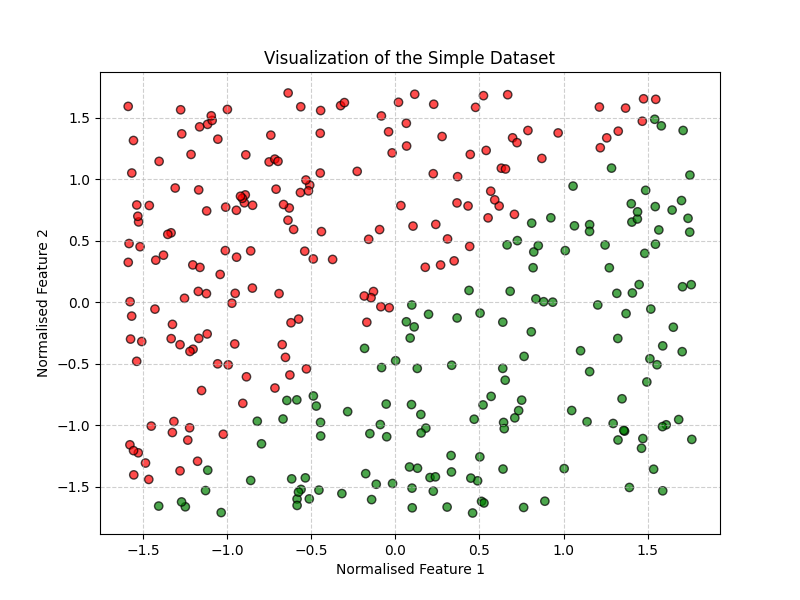
\includegraphics[width=0.7\linewidth]{simpledata.png}
    \caption{Scatter plot of the \texttt{simple} dataset, demonstrating linear separability.}
    \label{fig:simple_data}
\end{figure}

Upon inspection of the resulting plot, the dataset consists of two clearly seperated clusters. Due to the fact that a straight line can be drawn to 
perfectly divide the two classes without any overlap, this dataset is classified as linearly seperable. On account of this, the single-layer perceptron 
(using a linear transformation and sigmoid activation) implemented in this section, is sufficient to achieve optimal classification performance.

\subsection*{Forward pass}
The forward pass is the fundamental process by which the network transforms input data into a prediction. For the single layer implemented in this section, 
a linear layer output, $z_i$, and then the activation function output $v_i$ is calculated. As demonstrated in Listing \ref{lst:forwardpass} below, 
$z_i$ is computed by performing a matrix multiplication between the transpose of the weight matrix $W$ and the input vector $u_i$ (including a bias term). 
Following the linear transformation, the sigmoid activation function is applied to $z_i$ to produce the final activation output, $v_i$. 

\newpage
\begin{lstlisting}[
    language=Python, 
    caption={Implementation of the forward pass for a single layer},
    label={lst:forwardpass},
    breaklines=true,
    basicstyle=\ttfamily\small,
    frame=single
]
z_i = W.T @ u_i  # Linear layer output (Transpose W to match dimensions for matrix multiplication)
v_i = sigmoid(z_i) # Activation function output
return z_i, v_i
\end{lstlisting}

\subsection*{Loss derivative}
The optimisation of the network relies on the calculation of the gradient of the loss function (Binary Cross-Entropy) with respect to the model's 
predictions $\hat{y}$. This derivative serves as the initial error signal, Lambda, that is propagated backward through the network.
As shown in the Listing \ref{lst:logderiv} implementation below, the derivative of the binary cross-entropy loss is calculated using the following formula.
\begin{equation}
    \frac{\partial L}{\partial \hat{y}} = \frac{y - \hat{y}}{\hat{y}(1 - \hat{y}) + \epsilon}
    \label{eq:bce_derivative}
\end{equation}
To ensure numerical stability and prevent a division-by-zero error when $\hat{y}$ is exactly 0 or 1, a small constant $\epsilon$ ($1 \times 10^{-7}$) is added to the denominator. 

\begin{lstlisting}[
    language=Python, 
    caption={Implementation of the derivative of the binary cross-entropy},
    label={lst:logderiv},
    breaklines=true,
    basicstyle=\ttfamily\small,
    frame=single
]
eps = 1e-7
dL_dy_hat = None
dL_dy_hat = (y - y_hat) / (y_hat * (1 - y_hat) + eps)  # Add eps to avoid division by zero
return dL_dy_hat
\end{lstlisting}

\subsection*{Backward pass}
The backward pass is the mechanism by which the network propagates the error signal from the output layer back toward the input, enabling the update 
of the weights via gradient descent. This process begins by computing the gradient of the loss with respect to the linear output $z_i$, where $\Lambda$ is 
the error signal. 

\begin{equation}
\delta_i = \Lambda \odot v_i(1 - v_i)
\label{eq:local_gradient}
\end{equation}

This result is subsequently used to determine the gradient of the loss with respect to the weights, $\frac{\partial J}{\partial W_i}$. 

\begin{equation}
\frac{\partial J}{\partial W_i} = u_i \delta_i
\label{eq:weight_gradient}
\end{equation}

A new $\Lambda$ is then calculated to be passed to the preceeding layer. However this is only necessary for deeper architectures, where more than one layer 
makes up the network. When this updated $\Lambda$ is computed, the first row of the weight matrix $W_i$ is excluded since this row exists to incorporate a bias term and 
does not receive an error signal from previous layers. Listing \ref{lst:backpass} shows the necessary code to execute the backpass functionality.

\begin{lstlisting}[
    language=Python, 
    caption={Implementation of the backward pass},
    label={lst:backpass},
    breaklines=true,
    basicstyle=\ttfamily\small,
    frame=single
]
delta = Lambda * v_i * (1 - v_i)  # Backpropagation factor for layer i (Q_i,1)
dJ_dWi = u_i @ delta.T  # Gradients of weights for layer i
Lambda = (W_i[1:, :] @ delta).flatten() # Backpropagation factor for previous layer (Q_i,1) 
return dJ_dWi,Lambda
\end{lstlisting}

\subsection*{Model training}
Following the implementation of the forward and backward passes, the model was trained for 100 epochs using the default hyperparameters (learning rate of 0.1 and batch size of 1). 
Based on the training output, the model performance evolved as follows:
\begin{enumerate}
  \item Epoch 0: test loss of -0.1529
  \item Epoch 99: test loss of -0.0205
\end{enumerate}
Table \ref{tab:final_epochsq1} illustrates model output over the last 10 epochs of training.
\clearpage
\begin{table}[htbp]
    \centering
    \caption{Training and test loss for the final 10 epochs of the single-layer perceptron on the \texttt{simple} dataset.}
    \label{tab:final_epochsq1}
    \begin{tabular}{ccc}
        \hline
        \textbf{Epoch} & \textbf{Training Loss} & \textbf{Test Loss} \\ \hline
        90 & -0.0363 & -0.0204 \\
        91 & -0.0362 & -0.0200 \\
        92 & -0.0361 & -0.0208 \\
        93 & -0.0359 & -0.0218 \\
        94 & -0.0358 & -0.0220 \\
        95 & -0.0357 & -0.0214 \\
        96 & -0.0355 & -0.0202 \\
        97 & -0.0352 & -0.0195 \\
        98 & -0.0352 & -0.0202 \\
        99 & -0.0351 & -0.0205 \\ \hline
    \end{tabular}
\end{table}

In this specific implementation, a value closer to zero indicates higher likelihood and therefore a better model fit.
It is evident that the significant reduction in loss over model training demonstrates that the single-layer perceptron successfully converged. 

\subsection*{Model decision surface}
After training the model, the decision surface was visualised. The resulting plots, shown in Figure \ref{fig:decision_surface1} displays a clear, linear 
seperation between the two classes, which confirms that the single-layer perceptron has successfully learned to partition the data. 
\begin{figure}[htbp]
    \centering
    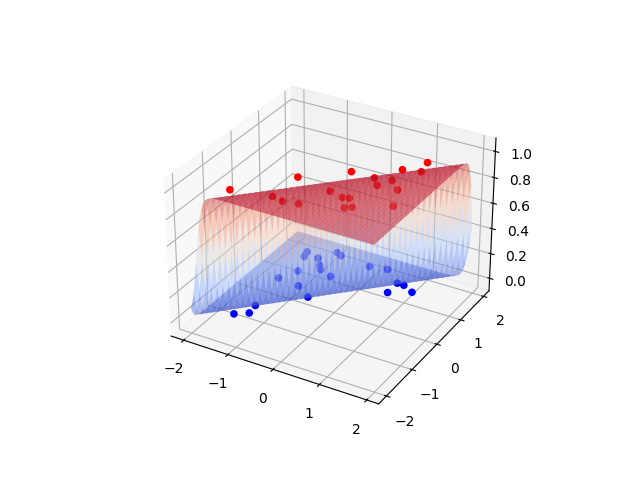
\includegraphics[width=0.7\linewidth]{decision_surface.png}
    \caption{Decision surface of the \texttt{simple} data}
    \label{fig:decision_surface1}
\end{figure}
It is important to note that the decision surface of a single-layer perceptron is linear. More complex decision boundaries can only be captured using multi-layer architectures. 
Considering the distribution of the \texttt{simple} dataset, as seen in Figure \ref{fig:simple_data}, a linear decision surface, and hence a single-layer perceptron, 
is sufficient to achieve optimal classification performance. 

\section*{Question 2: Multi-layer perceptron}

\subsection*{Data loading and visualisation}
The \texttt{two\_blob} dataset was loaded and visualised using the same approach as the \texttt{simple} dataset. The resulting scatter plot, shown in Figure \ref{fig:twoblob_data},
reveals a more complex distribution of data points, with two distinct clusters that are not linearly separable. This non-linear distribution necessitates the use of a multi-layer perceptron, which can capture more complex non-linear decision boundaries than a single-layer architecture.

\begin{figure}[htbp]
    \centering
    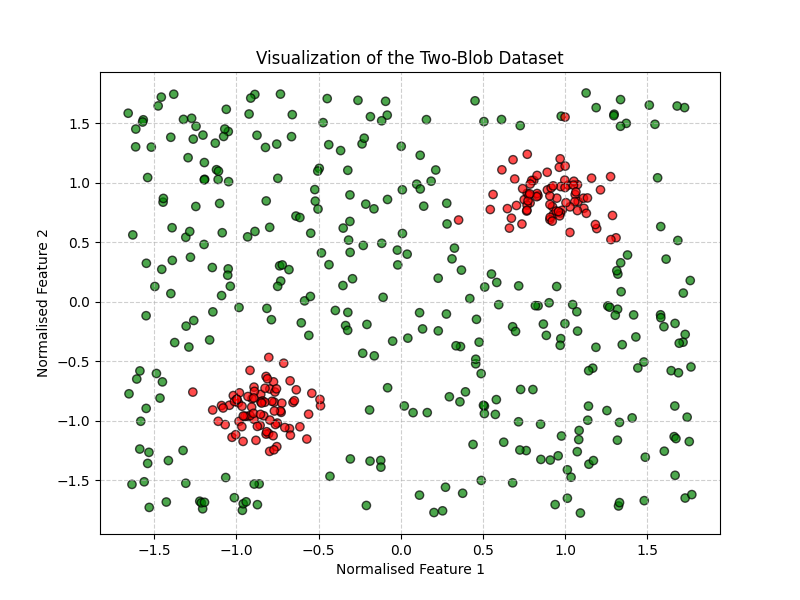
\includegraphics[width=0.7\linewidth]{twoblobdata.png}
    \caption{Scatter plot of the \texttt{two\_blob} dataset, demonstrating non-linear separability.}
    \label{fig:twoblob_data}
\end{figure}

\subsection*{Model architecture}
To address the non-linear nature of the \texttt{two\_blob} dataset, a multi-layer perceptron architecture was implemented. This architecture includes two extra layers 
$W_2$ and $W_3$ with dimensions $P2 = 8$, $P3 = 8$, and $Q3 = 1$ respectively. The weights are then initialised for all three layers.
Listing \ref{lst:mlt-layer} below shows the code used to define the dimensions of the multi-layer architecture.

\begin{lstlisting}[
    language=Python, 
    caption={Implementation of the multi-layer architecture},
    label={lst:mlt-layer},
    breaklines=true,
    basicstyle=\ttfamily\small,
    frame=single
]
P_1 = 2 # Input layer has two features
Q_1 = 8 # Number of neurons in first hidden layer = number of outputs

P_2 = 8 # Number of inputs to second hidden layer = number of neurons in first hidden layer
Q_2 = 8 # Number of neurons in second hidden layer = number of outputs

P_3 = 8 # Number of inputs to output layer = number of neurons in second hidden layer
Q_3 = 1 # Final output for binary classification

# Initialise weights for all three layers
W_1 = np.random.uniform(-1/np.sqrt(Q_1),1/np.sqrt(Q_1),size=(P_1+1,Q_1)) # initialise weights for layer W_1
W_2 = np.random.uniform(-1/np.sqrt(Q_2),1/np.sqrt(Q_2),size=(P_2+1,Q_2)) # initialise weights for layer W_2
W_3 = np.random.uniform(-1/np.sqrt(Q_3),1/np.sqrt(Q_3),size=(P_3+1,Q_3)) # initialise weights for layer W_3
\end{lstlisting}

\subsection*{Forward pass}
In a multi-layer architecture, the forward pass involves sequentially passing the input through each layer of the network. In this implementation, 
the data propagates through three weight matrices ($W_1$, $W_2$, and $W_3$). Since the weight matrices are designed to include a bias term, a constant value of 1 is added to the activation vector 
$v_i$ using a vertical stacking operation to form the input vector $u_{i+1}$ for the following layer. Listing \ref{lst:forwardpass_mlt} below demonstrates the implementation of the forward pass for the multi-layer architecture.
The forward pass follows a chain: the features $u_1$ produce activations $v_1$ in the first hidden layer, which are then used to compute the activations $v_2$ in the second hidden layer, and finally the output $y\_hat$ is generated from the activations of the last layer.

\begin{lstlisting}[
    language=Python, 
    caption={Implementation of the forward pass for the multi-layer architecture},
    label={lst:forwardpass_mlt},
    breaklines=true,
    basicstyle=\ttfamily\small,
    frame=single
]
u_1 = np.hstack([np.ones((1,1)),train_X[i:(i+1),:]]).T # extract i'th input from training set and add bias
z_1,v_1 = forward(u_1,W_1) # calculate z_i and v_i for layer 1
u_2 = np.vstack([np.ones((1, 1)), v_1]) # Add bias to the input of the second layer
z_2, v_2 = forward(u_2, W_2)  # Calculate z_i and v_i for layer 2
u_3 = np.vstack([np.ones((1,1)), v_2]) # Add bias to the input of the third layer
z_3, v_3 = forward(u_3, W_3) # Calculate z_i and v_i for layer 3
y_hat = v_3 # Final prediction is the activation of the last layer
\end{lstlisting}

\subsection*{Backward pass}
The backpropagation process involves calculating the gradients for each layer, starting from the output layer and moving backward through the network. In this implementation, 
the error signal $\Lambda$ is initialised using the derivative of the binary cross-entropy loss and is iteratively updated at each layer. This iterative process ensures 
that each weight matrix receives the appropriate gradient information as described in the following equation.
\begin{equation}
    \frac{\partial J}{\partial W_i} = \underbrace{\frac{\partial z_i}{\partial W_i}}_{u_i} \cdot \underbrace{\frac{\partial v_i}{\partial z_i}}_{\sigma'(z_i)} \cdot {\Lambda}
    \label{eq:chain_rule_expansion}
\end{equation}
The gradients for each layer are accumulated in the \texttt{avg\_grads} list, which is used to update the weights after processing a batch of data. 
The weights are updated using a gradient descent step as described by the following formula:
\begin{equation}
    W_i = W_i - \alpha \cdot \frac{\partial J}{\partial W_i}
    \label{eq:weight_update}    
\end{equation}
In this equation, $\alpha$ represents the learning rate. Listing \ref{lst:backpass_mlt} below demonstrates the implementation of the backward pass for the multi-layer architecture.
\begin{lstlisting}[
    language=Python, 
    caption={Implementation of the backward pass for the multi-layer architecture},
    label={lst:backpass_mlt},
    breaklines=true,
    basicstyle=\ttfamily\small,
    frame=single
]
Lambda = loss_derivative(y,y_hat) # initialise Lambda
dJ_dw3, Lambda = backward(u_3, v_3, W_3, Lambda) # Calculate derivatives for layer 3 by backpropagation
avg_grads[2] += dJ_dw3 # accumulate gradients for W_3
dJ_dw2, Lambda = backward(u_2, v_2, W_2, Lambda) # Calculate derivatives for layer 2 by backpropagation
avg_grads[1] += dJ_dw2 # accumulate gradients for W_2
dJ_dw1,Lambda = backward(u_1,v_1,W_1,Lambda) # calculate derivatives by backpropagation
avg_grads[0] += dJ_dw1 # accumulate gradients for W_1
\end{lstlisting}

\subsection*{Decision surface}
After training the multi-layer perceptron (with a learning rate of 0.1, 100 epochs and a batch size of 1) on the \texttt{two\_blob} dataset, test set loss is analysed and the decision surface is visualised. 
Based on the training output, the model performance evolved as follows:
\begin{enumerate}
  \item Epoch 0: test loss of -0.6572
  \item Epoch 99: test loss of -0.2042
\end{enumerate}
Table \ref{tab:final_epochsq2} illustrates model output over the last 10 epochs of training, whereas the plot, shown in Figure \ref{fig:decision_surface2}, displays the non-linear decision boundary that effectively separates the two classes.

\begin{table}[htbp]
    \centering
    \caption{Training and test loss for the final 10 epochs of the single-layer perceptron on the \texttt{two\_blob} dataset.}
    \label{tab:final_epochsq2}
    \begin{tabular}{ccc}
        \hline
        \textbf{Epoch} & \textbf{Training Loss} & \textbf{Test Loss} \\ \hline
        90 & -0.1618 & -0.2166 \\
        91 & -0.1545 & -0.1885 \\
        92 & -0.1436 & -0.2212 \\
        93 & -0.1369 & -0.2294 \\
        94 & -0.1278 & -0.2491 \\
        95 & -0.1302 & -0.1579 \\
        96 & -0.1336 & -0.2296 \\
        97 & -0.1310 & -0.1639 \\
        98 & -0.1227 & -0.1945 \\
        99 & -0.1153 & -0.2042 \\ \hline
    \end{tabular}
\end{table}

\begin{figure}[htbp]
    \centering
    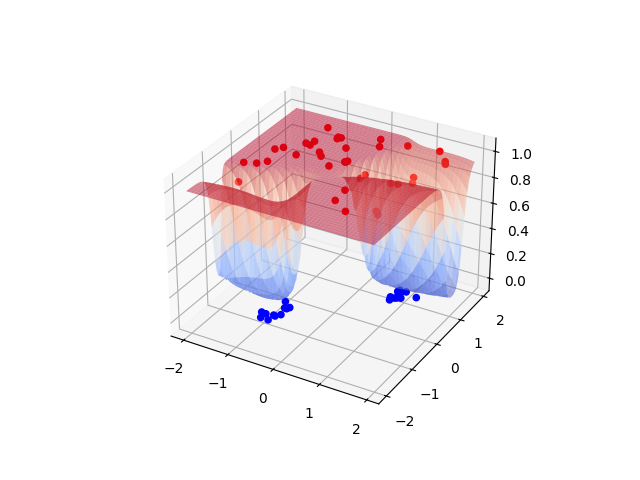
\includegraphics[width=0.7\linewidth]{decision_surface_q2.png}
    \caption{Decision surface of the multi-layer perceptron on the \texttt{two\_blob} dataset, demonstrating a non-linear decision boundary.}
    \label{fig:decision_surface2} 
\end{figure}
 
\newpage
The above results demonstrate that the multi-layer architecture has successfully learned to capture the complex patterns in the data, which a single-layer perceptron would not have been able to achieve.


\section*{Conclusion}
This practical successfully implemented both a single-layer and a multi-layer perceptron from fundamental principles to classify two different 
datasets. The following key conclusions can be made: 
\begin{itemize}
  \item The single-layer perceptron was sufficient to achieve optimal performance on the linearly separable \texttt{simple} dataset, as evidenced by the significant reduction in loss and the linear decision surface.
  \item The multi-layer perceptron was necessary to capture the non-linear patterns in the \texttt{two\_blob} dataset, as demonstrated by the non-linear decision boundary and the reduction in loss over training.
\end{itemize}

Ultimately, this practical highlights the power of stacking single linear perceptron units to create complex architectures capable of capturing highly complex classfication boundaries.

\end{document}
